\begin{enumerate}[\Large\bfseries 1.]

%----------1.
\item Encontrar el punto final de $\vec{a}=(7,6)$ si el punto inicial es $P_0(2,-1)$.\\\\
    Respuesta.-\; Sea $\vec{a}=P_1-P_0$ y $P_1=(x,y)$, entonces podemos hallar los vectores de la siguiente manera,
    \begin{center}
    \begin{tabular}{rcl}
	$x-2$&$=$&$7$\\
	$y+1$&$=$&$6$\\
    \end{tabular}
    \end{center}
    de donde $x=9, \; y=5$ y por lo tanto $$P_1=(9,5)$$\\

%----------2.
\item Sean $\vec{u}=(1,3)$,  $\vec{v}=(2,1)$ y $\vec{w}=(4,-1)$. Encontrar las componentes del vector $\vec{x}$ que satisfacen $2\vec{u}-\vec{v}+\vec{x}=7\vec{x}+\vec{w}$.\\\\
    Respuesta.-\; Despejando $\vec{x}$ obtenemos $$6\vec{x}=2\vec{u}-\vec{v}-\vec{w} \quad \Longrightarrow\quad 6\vec{x}=(2,6)-(2,1)-(4,-1)$$ 
    de donde $$6\vec{x}=(0,5)-(4,-1)\quad \Longrightarrow \quad 6\vec{x}=(-4,6) \quad \Longrightarrow \quad \vec{x}=\left(-\dfrac{2}{3},1\right)$$\\

%----------3.
\item Demuéstrese que: $0\vec{x}=\vec{0}$ y $r\vec{0}=\vec{0}$.\\\\
    Demostración.-\; sea $\vec{x}\in V_n$ entonces $0\vec{x}=0(x_1,x_2,...,x_n)$, luego por la multiplicación de un número real por un vector tenemos, $$0\vec{x}=(0\cdot x_1,0\cdot x_2,...,0\cdot x_n)=(0,0,...,0)$$
    y por lo tanto se demuestra que $$0\vec{x}=\vec{0}$$\\
    Por otro lado sea $r\in \mathbb{R}$, por lo tanto $$r\vec{0}=r(0,0,...,0)=(r\cdot 0,r\cdot 0,...,r\cdot)=(0,0,...,0)$$
    de modo que $$r\vec{0}=\vec{0}$$\\

%----------4.
\item Demuéstrese que:
\begin{enumerate}[\bfseries a)]

    %-----a)
    \item Si $\vec{a}+\vec{b}=\vec{a}+\vec{c} \quad \Longrightarrow \quad \vec{b}=\vec{c}$.\\\\
	Demostración.-\; Sea $\vec{a},\vec{b},\vec{c} \in V_n$, entonces por el inverso aditivo en vectores e hipótesis tenemos ,
	\begin{center}
	    \begin{tabular}{rcl}
		$\vec{b}$&$=$&$(\vec{b}+\vec{a})-\vec{a}$\\
		&$=$&$(\vec{a}+\vec{b})-\vec{a}$\\
		&$=$&$(\vec{a}+\vec{c})-\vec{a}$\\
		&$=$&$\vec{c}+(\vec{a}-\vec{a})$\\
		&$=$&$\vec{c}$\\\\
	    \end{tabular}
	\end{center}

    %-----b)
    \item Si $r\vec{x}=\vec{0}\quad \Longrightarrow \quad r=0 \lor \vec{x}=\vec{0}$.\\\\
	Demostración.-\; Será lo mismo demostrar $r\vec{x}=\vec{0}  \land r\neq 0\;\Longrightarrow\;\vec{x}=\vec{0}$. Esto por leyes lógicas.\\\\
	Sea $r\in \mathbb{R}$ y $\vec{x} \in V_n$, entonces $$r\vec{x}=0 \;\; \mbox{implica que}\;\;  \vec{x}=\dfrac{\vec{0}}{r}, \;\; \mbox{ya que}\;\; r\neq 0.$$ Luego se sigue que $$\vec{x}=\vec{0}$$\\

    %-----c)
    \item Si $r\vec{x}=s\vec{x}\;\land\; \vec{x}\neq 0 \quad \Longrightarrow \quad r=s$.\\\\
	Demostración.-\; Reescribiendo la proposición se tiene: Si $r\vec{x}=s\vec{x}\; \land \; r\neq s \;\; \Longrightarrow \; \; \vec{x}=0$.\\\\ 
	De donde se tiene $$\vec{x}=(r-s)\vec{x} \; \Longrightarrow \; \vec{x}=r\vec{x}-s\vec{x} \; \; \mbox{ya que }\; r\neq s$$ 
	y por lo tanto $$\vec{x}=r(\vec{x}-\vec{x})$$
	se sigue $$\vec{x}=r(0) \; \Longrightarrow \; \vec{x}=0$$
	debido a la unicidad y existencia del inverso aditivo. Con esto se demuestra la proposición dada.\\\\

\end{enumerate}

%----------5.
\item Demostrar que si $\vec{c}\neq 0$ y si $\vec{a}$ y $\vec{b}$ son paralelos a $\vec{c}$, entonces $\vec{a}$ y $\vec{b}$ son paralelos. (Vectores paralelos a un mismo vector no nulo son paralelos entre sí).\\\\
    Demostración.-\; Sea $\vec{a},\vec{b},\vec{c}\in V_n$. Por definición de vectores paralelos se tiene $$r_1\vec{a}=\vec{c}\quad \mbox{y} \quad r_2\vec{b}=\vec{c}$$ de donde $$r_1\vec{a}=r_2\vec{b},$$ en vista de que $r_1\cdot r_2 \neq 0$ entonces $$\vec{b}=r_1r_2^{-1} \vec{a},$$ por lo tanto se concluye que $\vec{a}$ y $\vec{b}$ son paralelos entre sí.\\\\

%----------6.
\item Hallar todos los vectores ortogonales a:
\begin{enumerate}[\bfseries a)]
    
    %-----a)
    \item $(3,6)$\\\\
	Respuesta.-\; Sea $(r_1,r_1)$ un vector, entonces para hallar vectores paralelos a $(3,6)$ utilizamos la definición como sigue,
	\begin{center}	
	    \begin{tabular}{rcl}
		$(3,6)\circ (r_1,r_2)$&$=$&$0$\\
		$3r_1+6r_2$&$=$&$0 \qquad$ producto escalar\\
		$3(r_1+2r_2)$&$=$&$0$\\
		$r_1+2r_2$&$=$&$0$\\
		$r_1$&$=$&$-2r_2$\qquad (1)\\
	    \end{tabular}
	\end{center}
	de donde tomamos valores para $r_2$, reemplazamos en (1) y obtendremos $n$ vectores paralelos a $(3,6)$.\\\\

    %-----b)
    \item $(2,-1)$.\\\\
	Respuesta.-\; Análogamente al inciso a) tenemos 
	\begin{center}
	\begin{tabular}{rcl}
	    $(2,-1)\circ (r_1,r_2)$&$=$&$0$\\
	    $2r_1 + (-r_2)$&$=$&$0$\\
	    $r_1$&$=$&$\frac{1}{2}r_2$\\
	\end{tabular}
	\end{center}
	de igual forma al anterior inciso, tomamos valores para $r_2$, y hallamos $n$ valores ortogonales a $(2,-1)$.\\\\

    %-----c)
    \item $(2,3,-1)$\\\\
	Respuesta.-\; Sea $(r_1,r_2,r_3)$ un vector en $V_3$, entonces, 
	\begin{center}
	\begin{tabular}{rcl}
	    $(2,3,-1)\circ (r_1,r_2,r_3)$&$=$&$0$\\
	    $2r_1+3r_2-r_3$&$=$&$0$\\
	    $r_1$&$=$&$(r_3-3r_2)/2 \qquad$ (1)\\
	\end{tabular}
	\end{center}
	luego reemplazamos valores a $r_3$ y $r_2$ en (1), de donde obtendremos vectores ortogonales a $(2,3,-1)$.\\\\

    %-----d)
    \item $(a_1,a_2)$\\\\
	Respuesta.-\; Análogo a los anteriores incisos se tiene,
	    $$(a_1,a_2)\circ (r_1,r_2)=0 \quad \Longrightarrow \quad 
	    a_1r_1 + a_2r_2=0 \quad \Longrightarrow \quad
	    \left\{ \begin{array}{l} a_1=-a_2r_2/r_1 \\ a_2=-a_1r_1/r_2 \\ r_1=-a_2r_2/a_1 \\ r_2=-a_1r_1/a_1 \end{array}\right.$$

	    \vspace{.6cm}

\end{enumerate}

%----------7.
\item Encontrar un vector que sea ortogonal tanto a $\vec{u}$ como a $\vec{v}$.
\begin{enumerate}[\bfseries a)]

    %-----a)
    \item $\vec{u}=-7i+3j+k, \quad \vec{v}=2i+4k$.\\\\
	Respuesta.-\;
	$$\vec{u}\times \vec{v} = \left|\begin{array}{ccc}
	    i&j&k\\
	    7&3&1\\
	    2&0&4\\
	\end{array}\right|=\left|\begin{array}{cc}3&1\\ 0&4 \end{array}\right|i - \left|\begin{array}{cc} 7&1\\2&4 \end{array}\right|j + \left|\begin{array}{cc} 7&3\\2&0 \end{array}\right|k=(3\cdot 4 - 1\cdot 0)i - (7\cdot 4-2\cdot 1)j+(7\cdot 0 - 3\cdot 2)k$$
	y por lo tanto el vector que deseamos encontrar es $$\vec{u}\times \vec{v}=(12,-26,-6)$$\\

    %-----b)
    \item $\vec{u}=(-1,-1,-1), \quad \vec{v}=(2,0,2)$\\\\
	Respuesta.-\;
	$$\vec{u}\times \vec{v} = \left|\begin{array}{rrr}
	    i&j&k\\
	    -1&-1&-1\\
	    2&0&2\\
	\end{array}\right|$$
	de donde $$\vec{u}\times \vec{v} = -2i +2k = (-2,0,2)$$\\

\end{enumerate}

%----------8.
\item Encontrar todos los vectores posibles de longitud $1$ ortogonales tanto a $\vec{a}=(3,-2,1)$ como a $\vec{b}=(-2,1,-3)$.\\\\
    Respuesta.-\;  Primeramente encontraremos el producto vectorial para luego utilizar el teorema $\dfrac{\vec{a}\times \vec{b}}{|\vec{a}\times \vec{b}|}=1$
    $$\vec{a}\times \vec{b} = \left|\begin{array}{rrr}
	i&j&k\\
	3&-2&1\\
	-2&1&-3\\
    \end{array}\right|=5i+7j-k=(5,7,-1).$$
    Luego $$|\vec{a}\times \vec{b}|=\sqrt{5^2+7^2+1^2}=5\sqrt{3}$$
    de donde, $$\dfrac{\vec{a}\times \vec{b}}{|\vec{a}\times \vec{b}|}=\left(\dfrac{1}{\sqrt{3}},\dfrac{7}{5\sqrt{3}},-\dfrac{1}{5\sqrt{3}}\right)$$
    por lo tanto los vectores de longitud $1$ ortogonales a $\vec{a}$ y $\vec{b}$, son $$\left(\dfrac{1}{\sqrt{3}},\dfrac{7}{5\sqrt{3}},-\dfrac{1}{5\sqrt{3}}\right) \qquad \mbox{y}\qquad \left(-\dfrac{1}{\sqrt{3}},-\dfrac{7}{5\sqrt{3}},\dfrac{1}{5\sqrt{3}}\right)$$
    El segundo vector cumple con la condición dada ya que es el vector contrario al encontrado primeramente.\\\\

%----------9.
\item Sean $\vec{a}=ti + j$ y $\vec{b}=4i+3j$. Encontrar el valor de $t$ tal que 
\begin{enumerate}[\bfseries a)]
    
    %-----a)
    \item $\vec{a}$ y $\vec{b}$ sean ortogonales.\\\\
	Respuesta.-\; Sea $\vec{a}=ti + j=(t,1)$ y $\vec{b}=4i+3j=(4,3)$, entonces por definición de ortogonalidad tenemos 
	$$\vec{a}\circ \vec{b} = 0 \;\; \Longrightarrow \; \; 4t+3=0 \;\; \Longrightarrow \; \; t=-3/4$$\\

    %-----b)
    \item El ángulo entre $\vec{a}$ y $\vec{b}$ sea $\pi/4$.\\\\
	Respuesta.-\; Aplicando $\vec{a}\circ \vec{b}=|\vec{a}||\vec{b}|\cos(\pi/4)$ tenemos, 
	$$4t+3=\sqrt{t^2+1}\cdot \sqrt{25}\cdot \dfrac{\sqrt{2}}{2} \;\; \Longrightarrow \; \; (4t^2+3)^2=(t^2+1)\cdot\dfrac{25}{2}\cdot \dfrac{1}{2}$$
	de donde se tiene $$7t^2+48-7=0$$
	se sigue $$t=\dfrac{1}{7} \quad \mbox{o}\quad t=-7$$\\

    %-----c)
    \item El ángulo entre $\vec{a}$ y $\vec{b}$ sea $\pi/6$.\\\\
	Respuesta.-\; Análogo al anterior ejercicio tenemos $$4t+3=\sqrt{t^2+1}\cdot \sqrt{25}\cdot \dfrac{\sqrt{3}}{2}\;\; \Longrightarrow \; \; (4t^2+3)^2=(t^2+1)\cdot\dfrac{25}{2}\cdot \dfrac{3}{4}\;\; \Longrightarrow \; \; -11t^2+96t-39=0$$
	de donde $$t=\dfrac{48+25\sqrt{3}}{11} \quad \mbox{o} \quad t=\dfrac{48-25\sqrt{3}}{11}$$\\

    %-----d)
    \item $\vec{a}$ y $\vec{b}$ sean paralelos.\\\\
	Respuesta.-\; Sea $\vec{a}=(t,1)$ y $\vec{b}=(4,3)$ entonces por definición de vectores paralelos tenemos que $$\vec{a}=c\vec{b} \quad \Longrightarrow \quad (t,1)=c(4,3) \quad \Longrightarrow \quad (t,1)=(4c,3c)$$
	de donde $$t=4c \qquad \mbox{y} \qquad 1=3c$$
	por lo tanto $c=\dfrac{1}{3}$. Se sigue $$t=\dfrac{4}{3}$$\\

\end{enumerate}

%----------10. 
\item Los vectores $\vec{a}$ y $\vec{b}$ forman un ángulo de $60^\circ$ con $\|\vec{a}\|=5,$ $\|\vec{b}\|=8$. Determinar $||\vec{a}-\vec{b}\|$ y $\|\vec{a}+\vec{b}\|$.\\\\
    Respuesta.-\; Sea $$\| \vec{a}\pm\vec{b}\|^2=\|a\|^2\|b\|^2 \pm 2\|\vec{a}\|\|\vec{b}\|\cos \theta$$  
    entonces se tiene, $$\|a\pm b\|^2 = 5^2 + 8^2 \pm 2\cdot 5\cdot 8 \cos\left(60\cdot\dfrac{\pi}{180}\right)$$
    por lo tanto $$\|\vec{a}-\vec{b}\| = 7 \qquad y \qquad \|\vec{a}+\vec{b}\| = \sqrt{129}$$\\

%----------11.
\item Los vectores $\vec{a}$ y $\vec{b}$ forman un ángulo de $30^\circ$ con $\|\vec{a}\|=1$, $\|\vec{b}\|=\sqrt{3}$. Calcular el ángulo formado por los vectores $\vec{a}+\vec{b}, \vec{a}-\vec{b}$.\\\\
    Respuesta.-\; Primero calculemos $$|\vec{a}-\vec{b}|^2 = 1^2 + \sqrt{3}^2 - 2\sqrt{3} \cos 30 = 1$$
    Luego calculamos el ángulo $\alpha$ asociado a $\vec{a}$ y $\vec{a}-\vec{b}$ de donde nos queda $$\alpha= \arccos \left(\dfrac{1^2+1^2-\sqrt{3}}{2}\right) = \arccos\left(\dfrac{2-\sqrt{3}}{2}\right) = 82\mbox{.}3$$
    Sea  $a+b$ la diagonal del paralelogramo formado por los lados $\vec{a}$ y $\vec{b}$ de donde el ángulo de $a+b$ será $15^\circ$. Por lo tanto  $a+b$ y  $a-b$ forman un ángulo de, $$180-82\mbox{.}3-15=82\mbox{.}7$$\\

%----------12.
\item Dados dos vectores $\vec{a},\vec{b}\vec{c}$ que satisfacen la condición $\vec{a}+\vec{b}+\vec{c} = \vec{0}$ y sabiendo que $\|\vec{a}\|=3, \|\vec{b}\|=1,\|\vec{a}\|=4$. Calcular $\vec{a}\cdot \vec{b}+\vec{b}\cdot \vec{c}+\vec{a}\cdot \vec{c}$\\\\
    Respuesta.-\; Si $\vec{a}+\vec{b}+\vec{c}=0$ entonces $$0=\|\vec{0}\|^2=\|\vec{a}+\vec{b}+\vec{c}\|^2.$$ Luego $$\|\vec{a}\|^2 + \|\vec{b}\|^2 + \|\vec{c}\|^2 + 2(\vec{a}\cdot \vec{b} + \vec{a}\cdot \vec{c} + \vec{b}\vec{c}) = 0$$
    de donde se tiene, $$ \vec{a}\cdot \vec{b} + \vec{a}\cdot \vec{c} + \vec{b}\vec{c} = 3^2 + 1^2 + 4^2 = 13.$$\\

%----------13.
\item Dados los puntos $P(3,4)$, $Q(1,1)$ y $R(5,2)$, usar métodos vectoriales para encontrar las coordenadas del cuarto vértice del paralelogramo cuyo lados adyacentes son $\vec{PQ}$ y $\vec{QR}$.\\\\
    Respuesta.-\; 

%----------14.
\item Demostrar que $(4,5,2),(4,7,9),(8,5,-6)$ son los vértices de un triángulo equilátero.\\\\
    Respuesta.-\; Supongamos que las distancias entre $A,B$ y $C$ son iguales, lo que implica que $|A-B|=|B-C|=|B-C|$, de donde 
    \begin{center}
	\begin{tabular}{ccccccc} 
	    $|A-B|$ & $=$ & $|(0,-2,-7)|$ & $=$ & $\sqrt{0^2+(-2)^2 + (-7)^2}$ & $=$ &$\sqrt{53}$\\\\
	    $|A-C|$ & $=$ & $|(-4,0,8)|$ & $=$ & $\sqrt{(-4)^2+0^2+8^2}$ & $=$ & $\sqrt{80}$\\\\  
	\end{tabular}
    \end{center}
    ya que $|A-B|\neq |A-C|$ se concluye que los puntos dado no son los vertices de un triangulo equilátero.\\\\ 

%----------15.

%----------16.
\item [\Large\bfseries 16.] Sean $\vec{a},\vec{b}\in \mathbb{R}$. Demuéstrese que $\|\vec{a}+\vec{b}\|^2-\|\vec{a}^2-\vec{b}\|^2=4\vec{a}\cdot \vec{b}$.\\\\
    Demostración.-\; Se tiene que $$\|\vec{a}+\vec{b}\|^2-\|\vec{a}^2-\vec{b}\|^2=|\vec{a}|^2 + 2\vec{a}\cdot \vec{b} + | \vec{b} |^2 - \left(|\vec{a}|^2 - 2\vec{a} \cdot \vec{b} + |\vec{b}^2|\right)=4\vec{a} \cdot \vec{b}$$\\

%----------17.

%----------18.
\item [\Large\bfseries 18.] Demostrar que: $\|\vec{a}+\vec{b}\|^2 + \|\vec{a}-\vec{b}\|^2 = 2\|\vec{u}\|^2+2\|\vec{v}\|^2$\\\\
    Demostración.-\; Análogamente al ejercicio 16 se tiene, 
    $$\|\vec{a}+\vec{b}\|^2 + \|\vec{a}-\vec{b}\|^2 = |\vec{a}|^2 + 2\vec{a}\cdot \vec{b} + |\vec{b}|^2 + |\vec{a}|^2 - 2\vec{a} \cdot \vec{b} + |\vec{b}^2| = 2|\vec{a}^2 + 2\|\vec{b}|^2$$\\

%----------19.

%----------20.
\item [\Large\bfseries 20.] Supóngase que $\vec{a}\cdot \vec{b} = \vec{a}\cdot \vec{c}$ y que $\vec{a}\neq 0$. Es posible inferir que $\vec{b}=\vec{c}$?. Explicar la respuesta.\\\\
    Respuesta.-\; Esta proposición es falsa ya que si $A=(1,1,1)$, $B=(1,-1,0)$ y $C=(0,-1,1)$ entonces $$A\cdot B = 1\cdot 1 + 1\cdot(-1)+1\cdot 0 = 0,$$ $$A\cdot C = 1\cdot 0 + 1\cdot(-1)+1\cdot 1 = 0$$
    de donde $B\neq C$.\\\\ 

%----------41.
\item [\Large\bfseries 41.] Demostrar vectorialmente la ley de cosenos.\\\\
    Demostración.-\; Supongamos que $\vec{a},\vec{b} \in V_n$ y, 
    \begin{center}
	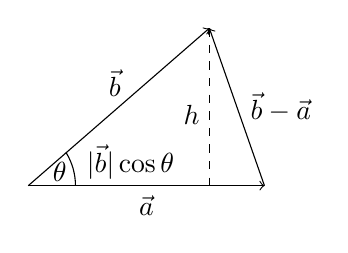
\begin{tikzpicture}
	    \draw[->](0,0)--(3,0);
	    \draw(1.5,0)node[below]{$\vec{a}$};
	    \draw[->](3,0)--(2.3,2);
	    \draw(1.1,1.3)node[]{$\vec{b}$};
	    \draw[<-](2.3,2)--(0,0);
	    \draw(2.7,1)node[right]{$\vec{b}-\vec{a}$};
	    \draw[dashed](2.3,2)--(2.3,0);
	    \draw(1.3,.3)node[]{$|\vec{b}|\cos \theta$};
	    \draw(2.3,.9)node[left]{$h$};
	    \draw(.4,.17)node[]{$\theta$};
	    \draw (0:.6cm) arc (0:32:.8cm);
	\end{tikzpicture}
    \end{center}
    entonces por el teorema de Pitágoras se tiene $$h^2=|\vec{b}|^2 - \left(|\vec{b}|\cos \theta\right)^2 \qquad y \qquad |\vec{b}-\vec{a}|^2 = \left(|\vec{b}|\cos \theta - |\vec{a}|\right)^2+h^2$$
    de donde $$|\vec{b}-\vec{a}|^2 = \left(|\vec{b}|\cos \theta - |\vec{a}|\right)^2+|\vec{b}|^2 - \left(|\vec{b}|\cos \theta\right)^2 = \left(|\vec{b}|\cos \theta\right)^2 - 2|\vec{a}||\vec{b}|\cos \theta + |\vec{a}|^2 + |\vec{b}|^2 - \left(|\vec{b}|\cos \theta\right)^2$$
    por lo tanto, $$|\vec{b}-\vec{a}|^2 = |\vec{a}|^2 + |\vec{b}|^2 - 2|\vec{a}||\vec{b}|\cos \theta $$\\

%----------42.

    


\end{enumerate}


